\documentclass[a4paper]{article}

\usepackage[english]{babel}
\usepackage{amsfonts, amssymb, mathtools, amsthm, amsmath}
\usepackage{graphicx, pgfplots}
\usepackage{bm} 
\usepackage{url}
\usepackage[dvipsnames]{xcolor}
\usepackage{lastpage}
\usepackage{chngcntr}
  \counterwithin{figure}{section}
  \renewcommand{\thefigure}{\thesection.\arabic{figure}}

%loaded last
\usepackage[hidelinks]{hyperref}
\usepackage[nameinlink]{cleveref} 

\usepackage{siunitx}
  \sisetup{exponent-product = \cdot,
    output-decimal-marker = {,}}

%Giles Castelles incfig
\usepackage{import}
\usepackage{xifthen}
\usepackage{pdfpages}
\usepackage{transparent}

\newcommand{\incfig}[2][1]{%
  \def\svgwidth{#1\columnwidth}
  \import{./figures/}{#2.pdf_tex}
}

\setlength{\parindent}{0in}
\setlength{\parskip}{12pt}
\setlength{\oddsidemargin}{0in}
\setlength{\textwidth}{6.5in}
\setlength{\textheight}{8.8in}
\setlength{\topmargin}{0in}
\setlength{\headheight}{18pt}

\usepackage{fancyhdr}
\pagestyle{fancy}

\fancyhead{}
\fancyfoot{}
\fancyfoot[R]{\thepage}
\fancyhead[C]{\leftmark}

\pgfplotsset{compat=newest}

\pgfplotsset{every axis/.append style={
  axis x line=middle,    % put the x axis in the middle
  axis y line=middle,    % put the y axis in the middle
  axis line style={<->,color=black}, % arrows on the axis
}}

\usepackage{thmtools}
\usepackage{tcolorbox}
  \tcbuselibrary{skins, breakable}
  \tcbset{
    space to upper=1em,
    space to lower=1em,
  }

\theoremstyle{definition}

\newtcolorbox[auto counter]{definition}[1][]{%
  breakable,
  colframe=ForestGreen,  %frame color
  colback=ForestGreen!5, %background color
  colbacktitle=ForestGreen!25, %background color for title
  coltitle=ForestGreen!70!black,  %title color
  fonttitle=\bfseries\sffamily, %title font
  left=1em,              %space on left side in box,
  enhanced,              %more options
  frame hidden,          %hide frame
  borderline west={2pt}{0pt}{ForestGreen},  %display left line
  title=Definition \thetcbcounter: #1,
}

\newtcolorbox{greenline}{%
  breakable,
  colframe=ForestGreen,  %frame color
  colback=white,          %remove background color
  left=1em,              %space on left side in box
  enhanced,              %more options
  frame hidden,          %hide frame
  borderline west={2pt}{0pt}{ForestGreen},  %display left line
}

\newtcolorbox[auto counter, number within=section]{dis}[1][]{%
  breakable,
  colframe=NavyBlue,  %frame color
  colback=NavyBlue!5, %background color
  colbacktitle=NavyBlue!25,    %background color for title
  coltitle=NavyBlue!70!black,  %title color
  fonttitle=\bfseries\sffamily, %title font
  left=1em,            %space on left side in box,
  enhanced,            %more options
  frame hidden,        %hide frame
  borderline west={2pt}{0pt}{NavyBlue},  %display left line
  title=Discussion \thetcbcounter: #1
}

\newtcolorbox{blueline}{%
  breakable,
  colframe=NavyBlue,     %frame color
  colback=white,         %remove background
  left=1em,              %space on left side in box,
  enhanced,              %more options
  frame hidden,          %hide frame
  borderline west={2pt}{0pt}{NavyBlue},  %display left line
}

\newtcolorbox{exa}[1][]{%
  breakable,
  colframe=RawSienna,  %frame color
  colback=RawSienna!5, %background color
  colbacktitle=RawSienna!25,    %background color for title
  coltitle=RawSienna!70!black,  %title color
  fonttitle=\bfseries\sffamily, %title font
  left=1em,              %space on left side in box,
  enhanced,              %more options
  frame hidden,          %hide frame
  borderline west={2pt}{0pt}{RawSienna},  %display left line
  title=Example: #1,
}

\newtcolorbox[auto counter, number within=section]{sæt}[1][]{%
  breakable,
  colframe=RawSienna,  %frame color
  colback=RawSienna!5, %background color
  colbacktitle=RawSienna!25,    %background color for title
  coltitle=RawSienna!70!black,  %title color
  fonttitle=\bfseries\sffamily, %title font
  left=1em,              %space on left side in box,
  enhanced,              %more options
  frame hidden,          %hide frame
  borderline west={2pt}{0pt}{RawSienna},  %display left line
  title=Sætning \thetcbcounter: #1,
  before lower={\textbf{Bevis:}\par\vspace{0.5em}},
  colbacklower=RawSienna!25,
}

\newtcolorbox{redline}{%
  breakable,
  colframe=RawSienna,  %frame color
  colback=white,       %Remove background color
  left=1em,            %space on left side in box,
  enhanced,            %more options
  frame hidden,        %hide frame
  borderline west={2pt}{0pt}{RawSienna},  %display left line
}

\newtcolorbox{des}[1][]{%
  breakable,
  colframe=NavyBlue,  %frame color
  colback=NavyBlue!5, %background color
  colbacktitle=NavyBlue!25,    %background color for title
  coltitle=NavyBlue!70!black,  %title color
  fonttitle=\bfseries\sffamily, %title font
  left=1em,              %space on left side in box,
  enhanced,              %more options
  frame hidden,          %hide frame
  borderline west={2pt}{0pt}{NavyBlue},  %display left line
  title=Description of #1,
}

\makeatother
\def\@lecture{}%
\newcommand{\lecture}[3]{
  \ifthenelse{\isempty{#3}}{%
    \def\@lecture{Lecture #1}%
  }{%
    \def\@lecture{Lecture #1: #3}%
  }%
  \subsection*{\makebox[\textwidth][l]{\@lecture \hfill \normalfont\small\textsf{#2}}}
}

\makeatletter

\newcommand{\exercise}[1]{%
 \def\@exercise{#1}%
 \subsection*{Exercise #1}
}

\makeatother

%Format lim the same way in intext and in display
\let\svlim\lim\def\lim{\svlim\limits}

% horizontal rule
\newcommand\hr{
\noindent\rule[0.5ex]{\linewidth}{0.5pt}
}

\author{Noah Rahbek Bigum Hansen}



\title{Take-Home Assignment weeks 35--36}
\date{}

\begin{document}

\maketitle

\exercise{P1-1}
Determine the magnitude and coordinate direction angles of the resultant force acting at $A$.

\begin{figure} [ht]
  \centering
  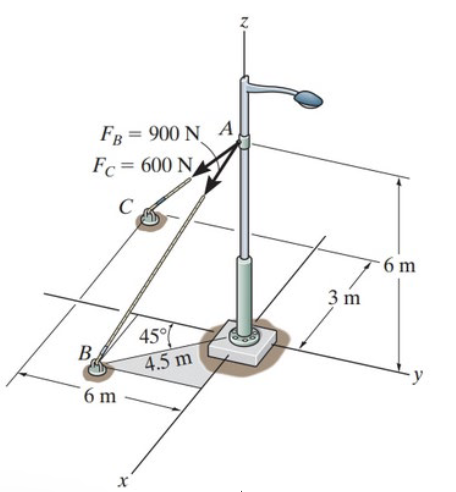
\includegraphics[width=0.35\linewidth]{../figures/P1_1}
\end{figure}

We start by adding a coordinate system such that the point $A$ is located at the origin $O$. The resultant force here $\textbf{F}_A$ is simply the sum of the two acting forces $F_B = \qty{900}{N}$ and $F_C = \qty{600}{N}$. We must therefore express these two in terms of Cartesian coordinates. First of all we start by determining the side length of the isoceles right triangle comprised by $\textbf{r}_B$ and its components. These components can be found as:
\[ 
  \cos \ang{45} \cdot \qty{4.5}{m} = \sin \ang{45} \cdot \qty{4.5}{m} = \qty{3,18}{m}
.\]
This means that the position vector $\textbf{r}_B$ can be written as:
\[ 
\textbf{r}_B = \left( \qty{3,18}{m} \textbf{i} - \qty{3,18}{m} \textbf{j} - \qty{6}{m} \textbf{k} \right)
.\]
A unit vector along this direction can be found as:
\[ 
\textbf{u}_B = \frac{\textbf{r}_B}{\left| \textbf{r}_B \right|} = \frac{ \left( \qty{3,18}{m} \textbf{i} - \qty{3,18}{m} \textbf{j} - \qty{6}{m} \textbf{k} \right)}{\sqrt{ \left( \qty{3,18}{m}  \right)^2 + \left( \qty{3,18}{m}  \right)^2 + \left( \qty{6}{m}  \right)^2 }} = \num{0,4241}  \textbf{i} - \num{0,4241}  \textbf{j} - \num{0,8002} \textbf{k}
.\]
Now if we just multiply this by the magnitude of the force $F_B$ we get the force in the direction of $B$ in cartestian coordinates:
\[ 
\textbf{F}_B = F_B \cdot \textbf{u}_B = \qty{900}{N} \cdot \left( \num{0,4241} \textbf{i} - \num{0,4241} \textbf{j} - \num{0,8002} \textbf{k}  \right) = \qty{381,69}{N} \, \textbf{i} - \qty{381,69}{N} \, \textbf{j} - \qty{720,18}{N} \, \textbf{k}
.\]

We can also find the unit vector along $\textbf{r}_C$ as:
\[ 
\textbf{u}_C = \frac{\textbf{r}_C}{\left| \textbf{r}_C \right|} = \frac{\left( - \qty{3}{m} \, \textbf{i} - \qty{6}{m} \, \textbf{j} - \qty{6}{m}\, \textbf{k} \right)}{\sqrt{\left( \qty{3}{m}  \right)^2 + \left( \qty{6}{m}  \right)^2 + \left( \qty{6}{m}  \right)^2}} = - \num{0,333} \textbf{i} - \num{0,666} \textbf{j} - \num{0,666} \textbf{k}
.\]
Therefore we can now find $\textbf{F}_C$ as:
\[ 
\textbf{F}_C = F_C \textbf{u}_C = \qty{600}{N} \cdot \left( -\num{0,333} \textbf{i} - \num{0,666} \textbf{j} - \num{0,666}  \textbf{k} \right) = - \qty{200}{N} \, \textbf{i} - \qty{400}{N} \, \textbf{j} - \qty{400}{N} \, \textbf{k}
.\]
The resultant force $\textbf{F}_A$ can now be found as:
\[ 
  \textbf{F}_A = \textbf{F}_B + \textbf{F}_C = \qty{0,182}{kN} \, \textbf{i} - \qty{0,782}{kN} \, \textbf{j} - \qty{1,12}{kN} \, \textbf{k}
.\]
The magnitude of this can be found by the Pythagorean theorem as:
\[ 
F_A = \sqrt{\left( \qty{0,182}{kN}  \right)^2 + \left( \qty{0,782}{kN}  \right)^2 +( \qty{1,12}{kN} )^2} = \qty{1,38}{kN} 
.\]
Now we can find the angles with each of the three axes as:
\begin{align*}
  \alpha &= \cos^{-1} \left( \frac{F_{Ax}}{F_A} \right) = \cos^{-1} \num{0,132} = \ang{82,4} \\
  \beta &= \cos^{-1} \left( \frac{F_{Ay}}{F_A} \right) = \cos^{-1} \num{-0,567} = \ang{124,5}  \\
  \gamma &= \cos^{-1} \left( \frac{F_{Az}}{F_A} \right) = \cos^{-1} \num{-0,813} = \ang{144,4} 
.\end{align*}
Therefore the resultant force $\textbf{F}_A$ is of magnitude \qty{1,38}{kN} and makes angles of \ang{82,4}, \ang{124,5}, and \ang{144,4} with the positive $x$-, $y$-, and $z$-axes respectively. 


\exercise{P2-1}
Determine the moment of the force of $F = \qty{600}{N}$ about point $A$.

\begin{figure} [ht]
  \centering
  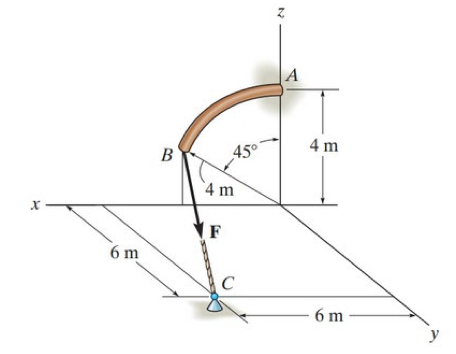
\includegraphics[width=0.35\linewidth]{../figures/P2_1.png}
\end{figure}
\bigbreak
The vector formulation of the moment is
\[ 
  \textbf{M}_A = \textbf{r} \times \textbf{F}
.\]
Where $\textbf{r}$ is the position vector between the point $A$ and any point on the line of action of $\textbf{F}$, e.g. $B$. Therefore
\[ 
  \textbf{r} = \textbf{r}_B - \textbf{R}_A = \left( 4 \cdot \sin \ang{45}, 0, 4 \cdot \cos \ang{45} \right) - \left( 0, 0, 4 \right) = \left( 2 \sqrt{2}, 0, 2 \sqrt{2} -4 \right) \unit{m}
.\]
The unit vector in the direction of $\textbf{F}$ is:
\[ 
  \textbf{u}_{F} = \frac{\textbf{C} - \textbf{B}}{C - B} = \frac{\left( 6 - 2 \sqrt{2}, 6, -2 \sqrt{2} \right)}{\sqrt{\left( 6 - 2 \sqrt{2} \right)^2 + 6^2 + \left( 2 \sqrt{2} \right)^2}} = \left( \num{0,4314}, \num{0,8161}, \num{-0,3847} \right)
.\]
And the force vector can thus be found as:
\[ 
  \textbf{F} = F \cdot \textbf{u}_F = \qty{600}{N} \cdot \left( \num{0,4314}, \num{0,8161}, \num{-0,3847}  \right) = \left( \num{258,82}, \num{489,63}, - \num{230,81} \right) \unit{N}
.\]
And the moment about $A$ is thus
\[ 
  \textbf{M}_A = \textbf{r} \times \textbf{F} = \left( 2 \sqrt{2}, 0, 2 \sqrt{2} - 4 \right) \unit{m} \cdot \left( \num{258,82}, \num{489,63}, - \num{230,81}   \right) \unit{N} = \left( \num{573,64}, \num{349,62}, \num{1384,89}  \right) \unit{N.m} 
.\]


\exercise{P2-2}
The friction at sleeve $A$ can provide a maximum resisting moment of \qty{125}{N.m} about the $x$-axis. Determine the largest magnitude of force $\textbf{F}$ that can be applied to the bracked so that the bracket will not turn.

\begin{figure} [ht]
  \centering
  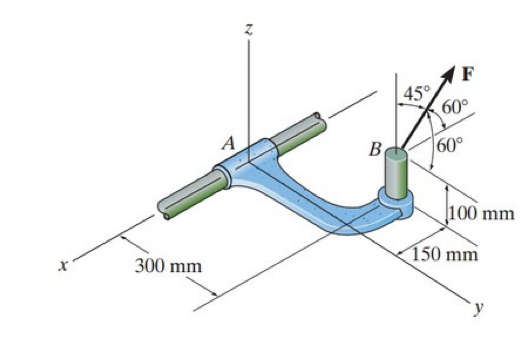
\includegraphics[width=0.35\linewidth]{../figures/P2_2.png}
\end{figure}
\bigbreak
Here, the same kind of reasoning is applied as above. We first find a position vector from the point of rotation $A$ to a point on the line of attack of the force $\textbf{F}$ at $B$. This is done as:
\[ 
\textbf{r} = \textbf{r}_B - \textbf{r}_{A} = \left( - 150, 300, 100 \right) \unit{mm} - \textbf{0} =  \left( - 150, 300, 100 \right) \unit{mm} 
.\]
Now we must find a unit vector in the direction of $\textbf{F}$, $\textbf{u}_F$. The drawing is a bit hard to decipher but it is understood as the force $\textbf{F}$ lying \ang{60} from the $-x$-axis, \ang{60} from the $+y$-axis, and \ang{45} from the $+z$-axis. Using the direction cosines we therefore get:
\begin{align*}
  \cos \alpha &= - \cos \ang{60} = - \num{0,5} \\
  \cos \beta &= \cos \ang{60} = \num{0,5}  \\
  \cos \gamma &= \cos \ang{45} = \num{0,7071} 
.\end{align*}
The unit vector of $\textbf{F}$ is therefore:
\[ 
\textbf{u}_F = \left( -\num{0,5} ; \num{0,5} ; \num{0,7071}  \right)
.\]

We have the following condition for the largest force the resisting friction can withstand:
\[ 
\textbf{M}_{A} = \textbf{r} \times \textbf{F} = \textbf{r} \times \left( \textbf{u}_F \cdot F \right)
.\]
We can solve this for the magnitude $F$ of the force $\textbf{F}$ as:
\begin{align*}
  \textbf{M}_A &= \textbf{r} \times \left( \textbf{u}_F \cdot F \right) \\
  \textbf{M}_A &= F \left( \textbf{r} \times \textbf{u}_F \right) \\
  F &= \frac{\textbf{M}_A}{\textbf{r} \times \textbf{u}_F}
.\end{align*}
And plugging in known values we get:
\[ 
F = \frac{\left( 125, 0, 0 \right) \unit{N.m}}{\left( - \num{0,15} ; \num{0,3} ; \num{0,1}  \right)\unit{m} \times \left( -\num{0,5} ; \num{0,5} ; \num{0,7071}  \right)} = \qty{771}{N}
.\]
Therefore the force $\textbf{F}$ should have a magnitude of at least $F = \qty{771}{N}$ before the friction force would not be able to hold the sleeve still. 


\exercise{P3-1}
Determine the magnitude and direction of $\theta$ of force $\textbf{F}$ and its displacement $d$ on the beam to that the loading system is equivalent to a resultant force of \qty{12}{kN} acting vertically downward at point $A$ and a clockwise couple moment of \qty{50}{kN.m}.

\begin{figure} [ht]
  \centering
  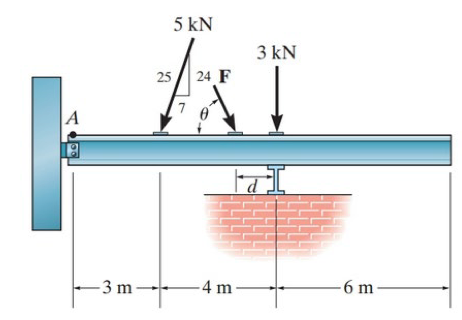
\includegraphics[width=0.5\linewidth]{../figures/P3_1.png}
\end{figure}
\bigbreak
The forces in the $x$- and $y$-directions can be expressed independently as:
\begin{align*}
  F_{x} &= \cos \theta F - \frac{7}{25} \cdot  \qty{5}{kN}  \\
  F_y &= - \left( \qty{3}{kN} + \frac{24}{25} \cdot  \qty{5}{kN} + \sin \theta F \right) 
.\end{align*}
The moments that each of the forces induce can also be expressed as (note that here clockwise is taken as the positive direction to simplify the calculations):
\[ 
M_A = \left( \qty{3}{m} \cdot \frac{24}{25} \cdot  \qty{5}{kN}  \right) + \left( \left( \qty{7}{m} - d \right) \cdot \sin \theta F \right) + \left( \qty{7}{m} \cdot \qty{3}{kN}  \right) 
.\]
We know that these, in static equilibrium will have the sizes $F_x = 0$, $F_y = -\qty{12}{kN}$ and $M_A = \qty{50}{kN m}$. We can therefore write:
\begin{align*}
  \cos \theta F &= \qty{1,4}{kN}  \\
  \sin \theta F &= \qty{12}{kN} - \qty{3}{kN} - \qty{4,8}{kN} = \qty{4,2}{kN}  \\
  \left( \qty{7}{m} - d \right) \cdot \sin \theta F &= \qty{50}{kN.m} - \left( \qty{3}{m} \cdot \qty{4,8}{kN} \right) - \qty{21}{kN.m} = \qty{14,6}{kN.m} 
.\end{align*}
By using the result for $\sin \theta F$ in the expression for the moment we can find $d$ as:
\begin{align*}
  \left( \qty{7}{m} - d \right)  &= \frac{\qty{14,6}{kN.m}}{\qty{4,2}{kN}} \\
  \qty{7}{m} - d &= \qty{3,47}{m} \\
  d &= \qty{7}{m} - \qty{3,47}{m} = \qty{3,52}{m} 
.\end{align*}
From the expressions for $\sin \theta F$ and $\cos \theta F$ we see that $\sin \theta F$ is 3 times as big. I.e.
\begin{align*}
  3 \cdot \cos \theta F &= \sin \theta F \\
  \cot \theta &= \frac{1}{3} \\
  \theta &= \cot^{-1} \frac{1}{3} = \ang{71,56}
.\end{align*}
And now the size $\textbf{F}$ is easily found as:
\[ 
F = \frac{\qty{1,4}{kN}}{\cos \ang{71,56} } = \qty{4,43}{kN}
.\]
Therefore $\textbf{F}$ is given as:
\[ 
\textbf{F} = \qty{4,43}{kN} \, \angle \, \ang{71,56}
\]
and it is applied at a distance $d = \qty{3,52}{m}$ from the support. 


\exercise{P3-2}
Replace the loading by an equivalent resultant force and couple moment acting at point $O$.

\begin{figure} [ht]
  \centering
  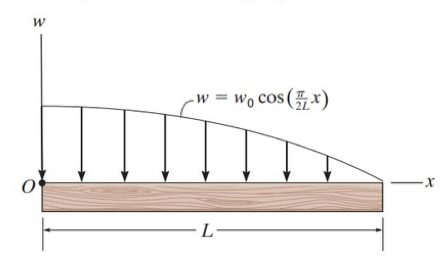
\includegraphics[width=0.5\linewidth]{../figures/P3_2.png}
\end{figure}
\bigbreak
The magnitude of the resultant force $F_R$ is obtained by integrating the distributed load over its entire length as:
\[ 
F_R = \int_L w(x) \, \mathrm{d}x
.\]
We therefore get:
\begin{align*}
  F_R &= \int_{0}^{L} w_0 \cos \left( \frac{\pi}{2L} x \right) \, \mathrm{d}x \\
      &= \left[ w_0 \cdot \frac{2L}{\pi} \sin \left( \frac{\pi}{2L} x \right) \right]_{0}^{L} \\
      &= w_0 \cdot \frac{2L}{\pi} \sin \left( \frac{\pi}{2} \right) - w_0 \frac{2L}{\pi} \sin 0 \\
      &= \frac{2L w_0}{\pi}
.\end{align*}
The magnitude of the resultant force is therefore $F = \frac{2L w_0}{\pi}$. This will act vertically downwards from the centroid, the $x$-coordinate $\overline{x}$ of which can be found as:
\[ 
\overline{x} = \frac{\int_L x w(x) \, \mathrm{d}x }{\int_L w(x) \, \mathrm{d}x}
.\]
We have already found the denominator of this so now we only need the numerator. For this we get:
\[ 
  w_0 \int_{0}^{L} x \cdot \cos \left( \frac{\pi}{2L}x \right)\, \mathrm{d}x = \frac{2 \left( \pi - 2 \right)L^2 w_0}{\pi^2}
.\]
And therefore $\overline{x}$ can now be determined as:
\begin{align*}
  \overline{x} &= \frac{2 \left( \pi - 2 \right)L^2 w_0 \cdot \pi}{\pi^2 2L w_0} \\
  &= \frac{\left( \pi - 2 \right)L}{\pi}
.\end{align*}
And thus the resultant moment is:
\[ 
M_O = \overline{x} F_R = \frac{(\pi - 2 ) L}{\pi} \cdot \frac{2 L w_0}{\pi} = \frac{2 \left( \pi - 2 \right)L^2 w_0}{\pi^2}
.\]
The equivalent resultant force and couple moment is therefore (following the standard conventions of $y$ being upwards and positive moment is counterclockwise):
\begin{align*}
  F_R &= -\frac{2L w_0}{\pi} \\
  M_O &= -\frac{2 \left( \pi - 2 \right) L^2 w_0}{\pi^2}
.\end{align*}


\exercise{P4-1}
The composite plate is made from both steel $(A)$ and brass $(B)$ segments. Determine the mass and location $(\overline{x}, \overline{y}, \overline{z})$ of its mass center $G$. Take $\rho_{\mathrm{st}} = \qty{7,85}{\frac{Mg}{m^3}} $ and $\rho_{\mathrm{br}} = \qty{8,74}{\frac{Mg}{m^3}}$. 
\begin{figure} [ht]
  \centering
  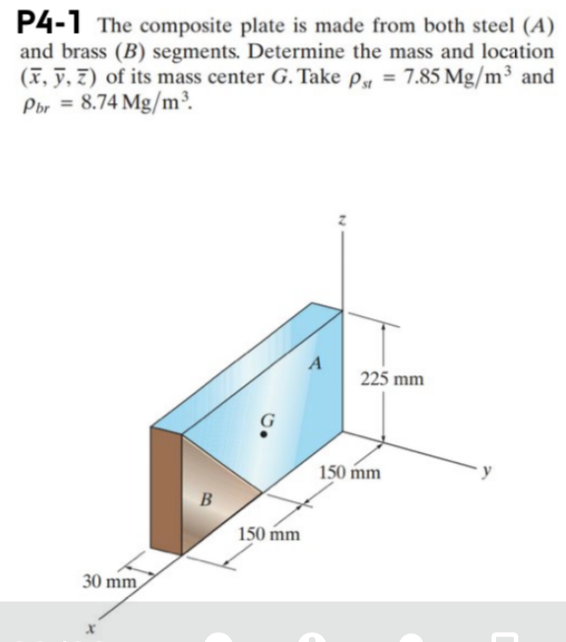
\includegraphics[width=0.5\linewidth]{../figures/p4_1.png}
\end{figure}
\bigbreak
We will consider the composite plate as if it consists of three distinct bodies. One rectangular steel segment, one triangular steel segment, and one triangular brass segment. The centroid of the rectangular steel segment, is placed ``half-way'' along each coordinate axis. I.e.
\begin{align*}
  \overline{x}_{A_1} &= \frac{\qty{150}{mm}}{2} = \qty{75}{mm}  \\
  \overline{y}_{A_1} &= \frac{- \qty{30}{mm} }{2} = - \qty{15}{mm}  \\
  \overline{z}_{A_1} &= \frac{\qty{225}{mm} }{2} = \qty{112,5}{mm} 
.\end{align*}
For the triangular sections we will first remember that the centroid of a triangular area is placed at $\frac{1}{3}$ of the height in each direction. I.e. for the triangular steel area:
\begin{align*}
  \overline{x}_{A_2} &= \qty{150}{mm} + \frac{\qty{150}{mm} }{3} = \qty{200}{mm}  \\
  \overline{z}_{A_2} &= \qty{225}{mm} - \frac{\qty{225}{mm} }{3} = \qty{150}{mm}
.\end{align*}
And as this area is homogeneous in the $y$-direction, the $y$-coordinate of the centroid must be in the middle of the segment in this direction. I.e.
\[ 
\overline{y}_{A_2} = -\frac{\qty{30}{mm} }{2} = -\qty{15}{mm} 
.\]
For the brass section we can follow the same reasoning and obtain:
\begin{align*}
  \overline{x}_{B} &= 2 \cdot \qty{150}{mm} - \frac{\qty{150}{mm} }{3} = \qty{250}{mm}  \\
  \overline{y}_B &= -\frac{\qty{30}{mm} }{2} = - \qty{15}{mm}   \\
  \overline{z}_B &= \frac{\qty{225}{mm} }{3} = \qty{75}{mm}
.\end{align*}
Now we must determine the mass of each segment using simple geometry as:
\begin{align*}
  m_{A_1} &= \qty{150}{mm} \cdot \qty{225}{mm} \cdot \qty{30}{mm} \cdot \qty{7,85}{\frac{Mg}{m^3}} = \qty{7,95}{kg}  \\
  m_{A_2} &= \frac{1}{2} \cdot m_{A_1} = \qty{3,98}{kg} \\
  m_{B} &= \frac{1}{2} \cdot \qty{150}{mm} \cdot \qty{225}{mm} \cdot \qty{30}{mm} \cdot \qty{8,74}{\frac{Mg}{m^3}} = \qty{4,42}{kg}
.\end{align*}
Now each coordinate of the center of gravity can be found as (note that as the centroid has a $y$-coordinate of \qty{-15}{mm} the center of gravity of the entire body will also be at this point in the $y$-direction):
\begin{align*}
  \overline{x} &= \frac{\sum \overline{x}_i W_i}{\sum W_i} \\
  &= \frac{\qty{75}{mm} \cdot \qty{7,95}{kg} + \qty{200}{mm} \cdot \qty{3,98}{kg} + \qty{250}{mm} \cdot \qty{4,42}{kg} }{\qty{7.95}{kg} + \qty{3,98}{kg} + \qty{4,42}{kg} } \\
  &= \qty{152,7}{mm} \\
  \overline{y} &= -\qty{15}{mm} \\
  \overline{z} &= \frac{\sum \overline{z}_i W_i}{\sum W_i} \\
  &= \frac{\qty{112,5}{mm} \cdot \qty{7,95}{kg} + \qty{150}{mm} \cdot \qty{3,98}{kg} + \qty{75}{mm} \cdot \qty{4,42}{kg} }{\qty{7,95}{kg} + \qty{3,98}{kg} + \qty{4,42}{kg} } \\
  &= \qty{111,5}{mm}
.\end{align*}
The entire weight of the body will be
\[ 
W = \qty{7,95}{kg} + \qty{3,98}{kg} + \qty{4,42}{kg} = \qty{16,35}{kg} 
.\]
And this will be acting from the center of gravity placed at $(\num{152,7}; \num{-15}; \num{111,5}) \, \unit{mm}$.



\end{document}
